\documentclass{beamer}
\let\vec\mathbf
\mode<presentation>
\usepackage{amsmath}
\usepackage{amssymb}
%\usepackage{advdate}
\usepackage{adjustbox}
%\usepackage{subcaption}
\usepackage{enumitem}
\usepackage{multicol}
\usepackage{mathtools}
\usepackage{listings}
\usepackage{url}
\usetheme{Boadilla}
\usecolortheme{lily}
\setbeamertemplate{footline}
{
  \leavevmode%
  \hbox{%
  \begin{beamercolorbox}[wd=\paperwidth,ht=2.25ex,dp=1ex,right]{author in head/foot}%
    \insertframenumber{} / \inserttotalframenumber\hspace*{2ex} 
  \end{beamercolorbox}}%
  \vskip0pt%
}
\setbeamertemplate{navigation symbols}{}
\providecommand{\nCr}[2]{\,^{#1}C_{#2}} % nCr
\providecommand{\nPr}[2]{\,^{#1}P_{#2}} % nPr
\providecommand{\mbf}{\mathbf}
\providecommand{\pr}[1]{\ensuremath{\Pr\left(#1\right)}}
\providecommand{\qfunc}[1]{\ensuremath{Q\left(#1\right)}}
\providecommand{\sbrak}[1]{\ensuremath{{}\left[#1\right]}}
\providecommand{\lsbrak}[1]{\ensuremath{{}\left[#1\right.}}
\providecommand{\rsbrak}[1]{\ensuremath{{}\left.#1\right]}}
\providecommand{\brak}[1]{\ensuremath{\left(#1\right)}}
\providecommand{\lbrak}[1]{\ensuremath{\left(#1\right.}}
\providecommand{\rbrak}[1]{\ensuremath{\left.#1\right)}}
\providecommand{\cbrak}[1]{\ensuremath{\left\{#1\right\}}}
\providecommand{\lcbrak}[1]{\ensuremath{\left\{#1\right.}}
\providecommand{\rcbrak}[1]{\ensuremath{\left.#1\right\}}}
\theoremstyle{remark}
\newtheorem{rem}{Remark}
\newcommand{\sgn}{\mathop{\mathrm{sgn}}}

\providecommand{\res}[1]{\Res\displaylimits_{#1}} 
\providecommand{\norm}[1]{\left\lVert#1\right\rVert}
\providecommand{\mtx}[1]{\mathbf{#1}}
\providecommand{\abs}[1]{\left\vert#1\right\vert}
\providecommand{\fourier}{\overset{\mathcal{F}}{ \rightleftharpoons}}
%\providecommand{\hilbert}{\overset{\mathcal{H}}{ \rightleftharpoons}}
\providecommand{\system}{\overset{\mathcal{H}}{ \longleftrightarrow}}
	%\newcommand{\solution}[2]{\textbf{Solution:}{#1}}
%\newcommand{\solution}{\noindent \textbf{Solution: }}align
\providecommand{\dec}[2]{\ensuremath{\overset{#1}{\underset{#2}{\gtrless}}}}
\newcommand{\myvec}[1]{\ensuremath{\begin{pmatrix}#1\end{pmatrix}}}
\usepackage{gensymb}

\title{Matrices in Geometry - 4.13.42}
\author{EE25BTECH11037  Divyansh}
\date{Sept, 2025}

\begin{document}

\maketitle


\section{Problem}
\begin{frame}
\frametitle{Problem Statement}
Let $0<\alpha<\frac{\pi}{2}$ be a fixed angle. If $\vec{P}=\brak{\cos{\theta},\  \sin{\theta}}$ and $\vec{Q} = \brak{\cos{\brak{\alpha - \theta}}, \ \sin{\brak{\alpha - \theta}}}$, then $\vec{Q}$ can be obtained from $\vec{P}$ by
\begin{enumerate}[label=(\alph*)]
    \item clockwise rotation around the origin through an angle $\alpha$
    \item anticlockwise rotation around the origin through an angle $\alpha$
    \item reflection in the line through origin with slope $\tan\alpha$
    \item reflection in the line through origin with slope $\tan\brak{\frac{\alpha}{2}}$
\end{enumerate}
\end{frame}

\section{Solution}
\begin{frame}{Solution}
   
We know that $\vec{Q}=\myvec{\cos{\brak{\alpha - \theta}} \\ \sin{\brak{\alpha - \theta}}}$ and $\vec{P}=\myvec{\cos{\theta}\\ \sin{\theta}}$
We also know that the rotation matrix $\vec{R}=\myvec{\cos\alpha & -\sin\alpha \\ \sin{\alpha} & \cos\alpha}$, where $\alpha$ is anticlockwise.
\\ We can obtain $\vec{Q}$ by
\begin{align}
    \vec{Q}=\vec{R}\vec{P} \implies \vec{Q}=\myvec{\cos\theta\cos\alpha - \sin\theta\sin\alpha \\ \sin\theta\cos\alpha +\cos\theta\sin\alpha   } 
\end{align}
We know from trigonometric identities that
\begin{align}
    \cos{\brak{\alpha-\theta}}=\cos\theta\cos\alpha + \sin\theta\sin\alpha \\\sin{\brak{\alpha-\theta}}=\cos\theta\sin\alpha - \sin\theta\cos\alpha
\end{align}
\end{frame}

\begin{frame}{Solution}
If we take $\alpha$ clockwise, that is, exchange it with $-\alpha$, we will get the rotation matrix as 
\begin{align}
    \vec{R}=\myvec{\cos\alpha & \sin\alpha \\ -\sin{\alpha} & \cos\alpha}
\end{align}
Thus, the required rotation matrix is $\vec{R}$ using which $\vec{Q}$ can be obtained from $\vec{P}$ by clockwise rotation around the origin through an angle $\alpha $, therefore the correct option is $\brak{a}$\\   
\end{frame}
\begin{frame}{Solution}
 Let us plot a graph for $\theta=45^{\degree}$ and $\alpha=30^{\degree}$
\begin{figure}[H]
    \centering
    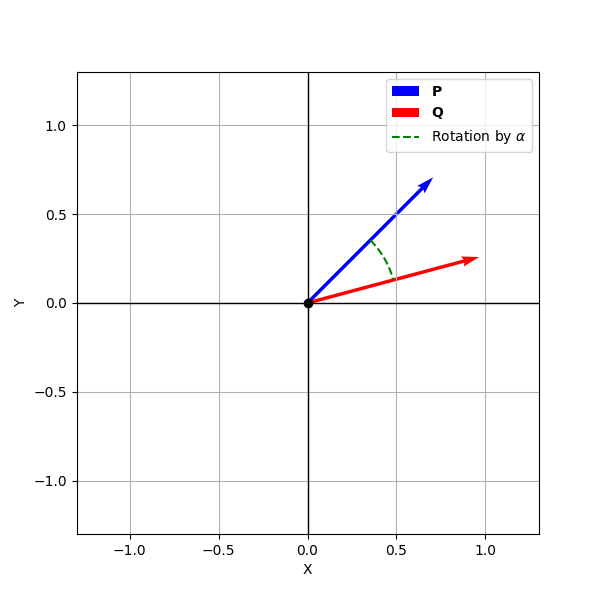
\includegraphics[width=0.5\columnwidth]{figs/1.png}
    \caption{Graph for 4.13.42}
    \label{fig:placeholder}
\end{figure}  
\end{frame}



\end{document}
